\documentclass[a4paper,12pt]{article}
\usepackage{czech}
\usepackage[utf8]{inputenc}
\usepackage{a4wide}
\usepackage[dvipdfm]{graphicx}
\usepackage{graphics}
\usepackage{indentfirst}
\usepackage{fancyhdr}
\usepackage{setspace}
\usepackage{amsmath}
\usepackage{amssymb}
\usepackage{epsfig}

%%\usepackage{nopageno}
%%\usepackage{txfonts}
\usepackage[usenames]{color}
\renewcommand{\d}{\mbox{d}}

\begin{document}
\section{Úkol}
\begin{enumerate}
\item   Proveďte energetickou kalibraci gama-spektrometru pomocí alfa zářiče $^{241}$Am.
\item   Určete materiál několika vzorků.
\item   Stanovte závislost účinnosti výtěžku rentgenového záření na atomovém čísle elementu v daném experimentálním uspořádání.
\item   Určete relativní zastoupené prvků v jednom ze vzorků.
\item   Na základě rentgenového záření identifikujte radioaktivní vzorek a stanovte typ pozorovaného rozpadu.
\end{enumerate}

\section{Teorie}
Za pomoci $\gamma$-zářiče je možné exitovat elektrony látky, kterou bychom chtěli určit. Tyto elektrony následně při návratu na původní hladinu vyzařují záření v rentgenové části spektra, které je pro ně charakteristické. Pokud změříme spoktrum tohoto záření, můžeme ho následně srovnatr s tabelovými hodnotami a následně určit zkoumaný prvek.

\section{Měření}
\subsection{Kalibrace}
Nejprve jsem za pomoci zářiče $^{241}$Am provedl kalibraci spektrometru. Ke kalibraci jsem využil známé hodnoty píků na energiích 59.5, 26.4 a 13.3 keV.

\subsection{Čisté kovy}
Nejprve jsem proměřil vzorky, které byli podle zadání čístými kovy. Jednalo se o vzorky číslo 1, 2, 3, 4, 6, 8, 9, 11a 12. V tabulce \ref{TKovy} jsou shrnuty výsledky měření spolus s tabelovými hodnotami odpovídajícími určený kovům.
Chyby intenzit jsou přibližně jedno procento.

\begin{table}
$$
\begin{array}{|c|c|c|c|}
\hline
&   E/\mbox{keV}&   E_t/\mbox{keV}&   \frac{S}{t}/\mbox{cps} \\ \hline
1 Cu&&& \\ \hline
K_{\alpha + \beta}& 8.15\pm 0.37&   8.027&   17.06 \\ \hline
2 Sn&&& \\ \hline
K_\alpha&   25.27\pm 0.38&  25.267&   68.27 \\ \hline
K_\beta&    28.61\pm 0.37&  28.481&   13.58 \\ \hline
3 Rh&&& \\ \hline
K_\alpha&   20.24\pm 0.34&  20.213&   36.45 \\ \hline
K_\beta&    20.8\pm 0.37&    22.720&   9.3 \\ \hline
4 Po&&& \\ \hline
L_\alpha&   10.63\pm 0.34&  10.550&   17.23 \\ \hline
L_\beta&    12.68\pm 0.36&  12.612&   14.16 \\ \hline
6 Zr&&& \\ \hline
K_\alpha&   15.82\pm 0.35&  15.690&   40.34 \\ \hline
K_\beta&    17.74\pm 0.35&  17.683&   9.91 \\ \hline
8 In&&& \\ \hline
K_\alpha&   24.22\pm 0.38&   24.206&   58.59 \\ \hline
K_\beta&   27.37\pm 0.41&   27.271&   13.50 \\ \hline
9 Mo&&& \\ \hline
K_\alpha&   17.52\pm 0.38&  17.374&   61.54 \\ \hline
K_\beta&    19.75\pm 0.39&  19.596&   14.37 \\ \hline
11 Cd&&& \\ \hline
K_\alpha&   23.18\pm 0.39&  23.170&   76.24 \\ \hline
K_\beta&    26.21\pm 0.36&  26.091&   18.40 \\ \hline
\end{array}
$$
\caption{Výslednky měření spektra pro čísté kovy.}
\label{TKovy}
\end{table}

Z naměřených ploch píků, které odpovídají intenzitě vzorku, jsem určil závislost výtěžku rentgenového záření na atomovém čísle prvku. Tato závislost je na obrázku (\ref{G1}). Tuto závislost jsem proložil polynomem pátého stupně, který má předpis
\begin{eqnarray}
f(Z)=-2.92e-5x^5+6.61e-3x^4-0.598x^3+27.0x^2-609x+5493
\end{eqnarray}

\begin{figure}
% GNUPLOT: LaTeX picture with Postscript
\begingroup
  \makeatletter
  \providecommand\color[2][]{%
    \GenericError{(gnuplot) \space\space\space\@spaces}{%
      Package color not loaded in conjunction with
      terminal option `colourtext'%
    }{See the gnuplot documentation for explanation.%
    }{Either use 'blacktext' in gnuplot or load the package
      color.sty in LaTeX.}%
    \renewcommand\color[2][]{}%
  }%
  \providecommand\includegraphics[2][]{%
    \GenericError{(gnuplot) \space\space\space\@spaces}{%
      Package graphicx or graphics not loaded%
    }{See the gnuplot documentation for explanation.%
    }{The gnuplot epslatex terminal needs graphicx.sty or graphics.sty.}%
    \renewcommand\includegraphics[2][]{}%
  }%
  \providecommand\rotatebox[2]{#2}%
  \@ifundefined{ifGPcolor}{%
    \newif\ifGPcolor
    \GPcolorfalse
  }{}%
  \@ifundefined{ifGPblacktext}{%
    \newif\ifGPblacktext
    \GPblacktexttrue
  }{}%
  % define a \g@addto@macro without @ in the name:
  \let\gplgaddtomacro\g@addto@macro
  % define empty templates for all commands taking text:
  \gdef\gplbacktext{}%
  \gdef\gplfronttext{}%
  \makeatother
  \ifGPblacktext
    % no textcolor at all
    \def\colorrgb#1{}%
    \def\colorgray#1{}%
  \else
    % gray or color?
    \ifGPcolor
      \def\colorrgb#1{\color[rgb]{#1}}%
      \def\colorgray#1{\color[gray]{#1}}%
      \expandafter\def\csname LTw\endcsname{\color{white}}%
      \expandafter\def\csname LTb\endcsname{\color{black}}%
      \expandafter\def\csname LTa\endcsname{\color{black}}%
      \expandafter\def\csname LT0\endcsname{\color[rgb]{1,0,0}}%
      \expandafter\def\csname LT1\endcsname{\color[rgb]{0,1,0}}%
      \expandafter\def\csname LT2\endcsname{\color[rgb]{0,0,1}}%
      \expandafter\def\csname LT3\endcsname{\color[rgb]{1,0,1}}%
      \expandafter\def\csname LT4\endcsname{\color[rgb]{0,1,1}}%
      \expandafter\def\csname LT5\endcsname{\color[rgb]{1,1,0}}%
      \expandafter\def\csname LT6\endcsname{\color[rgb]{0,0,0}}%
      \expandafter\def\csname LT7\endcsname{\color[rgb]{1,0.3,0}}%
      \expandafter\def\csname LT8\endcsname{\color[rgb]{0.5,0.5,0.5}}%
    \else
      % gray
      \def\colorrgb#1{\color{black}}%
      \def\colorgray#1{\color[gray]{#1}}%
      \expandafter\def\csname LTw\endcsname{\color{white}}%
      \expandafter\def\csname LTb\endcsname{\color{black}}%
      \expandafter\def\csname LTa\endcsname{\color{black}}%
      \expandafter\def\csname LT0\endcsname{\color{black}}%
      \expandafter\def\csname LT1\endcsname{\color{black}}%
      \expandafter\def\csname LT2\endcsname{\color{black}}%
      \expandafter\def\csname LT3\endcsname{\color{black}}%
      \expandafter\def\csname LT4\endcsname{\color{black}}%
      \expandafter\def\csname LT5\endcsname{\color{black}}%
      \expandafter\def\csname LT6\endcsname{\color{black}}%
      \expandafter\def\csname LT7\endcsname{\color{black}}%
      \expandafter\def\csname LT8\endcsname{\color{black}}%
    \fi
  \fi
  \setlength{\unitlength}{0.0500bp}%
  \begin{picture}(7200.00,5040.00)%
    \gplgaddtomacro\gplbacktext{%
      \csname LTb\endcsname%
      \put(1210,704){\makebox(0,0)[r]{\strut{} 0.19}}%
      \put(1210,1286){\makebox(0,0)[r]{\strut{} 0.2}}%
      \put(1210,1867){\makebox(0,0)[r]{\strut{} 0.21}}%
      \put(1210,2449){\makebox(0,0)[r]{\strut{} 0.22}}%
      \put(1210,3030){\makebox(0,0)[r]{\strut{} 0.23}}%
      \put(1210,3612){\makebox(0,0)[r]{\strut{} 0.24}}%
      \put(1210,4193){\makebox(0,0)[r]{\strut{} 0.25}}%
      \put(1210,4775){\makebox(0,0)[r]{\strut{} 0.26}}%
      \put(1342,484){\makebox(0,0){\strut{} 40}}%
      \put(2447,484){\makebox(0,0){\strut{} 42}}%
      \put(3553,484){\makebox(0,0){\strut{} 44}}%
      \put(4658,484){\makebox(0,0){\strut{} 46}}%
      \put(5764,484){\makebox(0,0){\strut{} 48}}%
      \put(6869,484){\makebox(0,0){\strut{} 50}}%
      \put(308,2739){\rotatebox{-270}{\makebox(0,0){\strut{}$K_\beta/K_\alpha$}}}%
      \put(4105,154){\makebox(0,0){\strut{}Z}}%
    }%
    \gplgaddtomacro\gplfronttext{%
      \csname LTb\endcsname%
      \put(3718,1097){\makebox(0,0)[r]{\strut{}data}}%
      \csname LTb\endcsname%
      \put(3718,877){\makebox(0,0)[r]{\strut{}fitovaný polynom}}%
    }%
    \gplbacktext
    \put(0,0){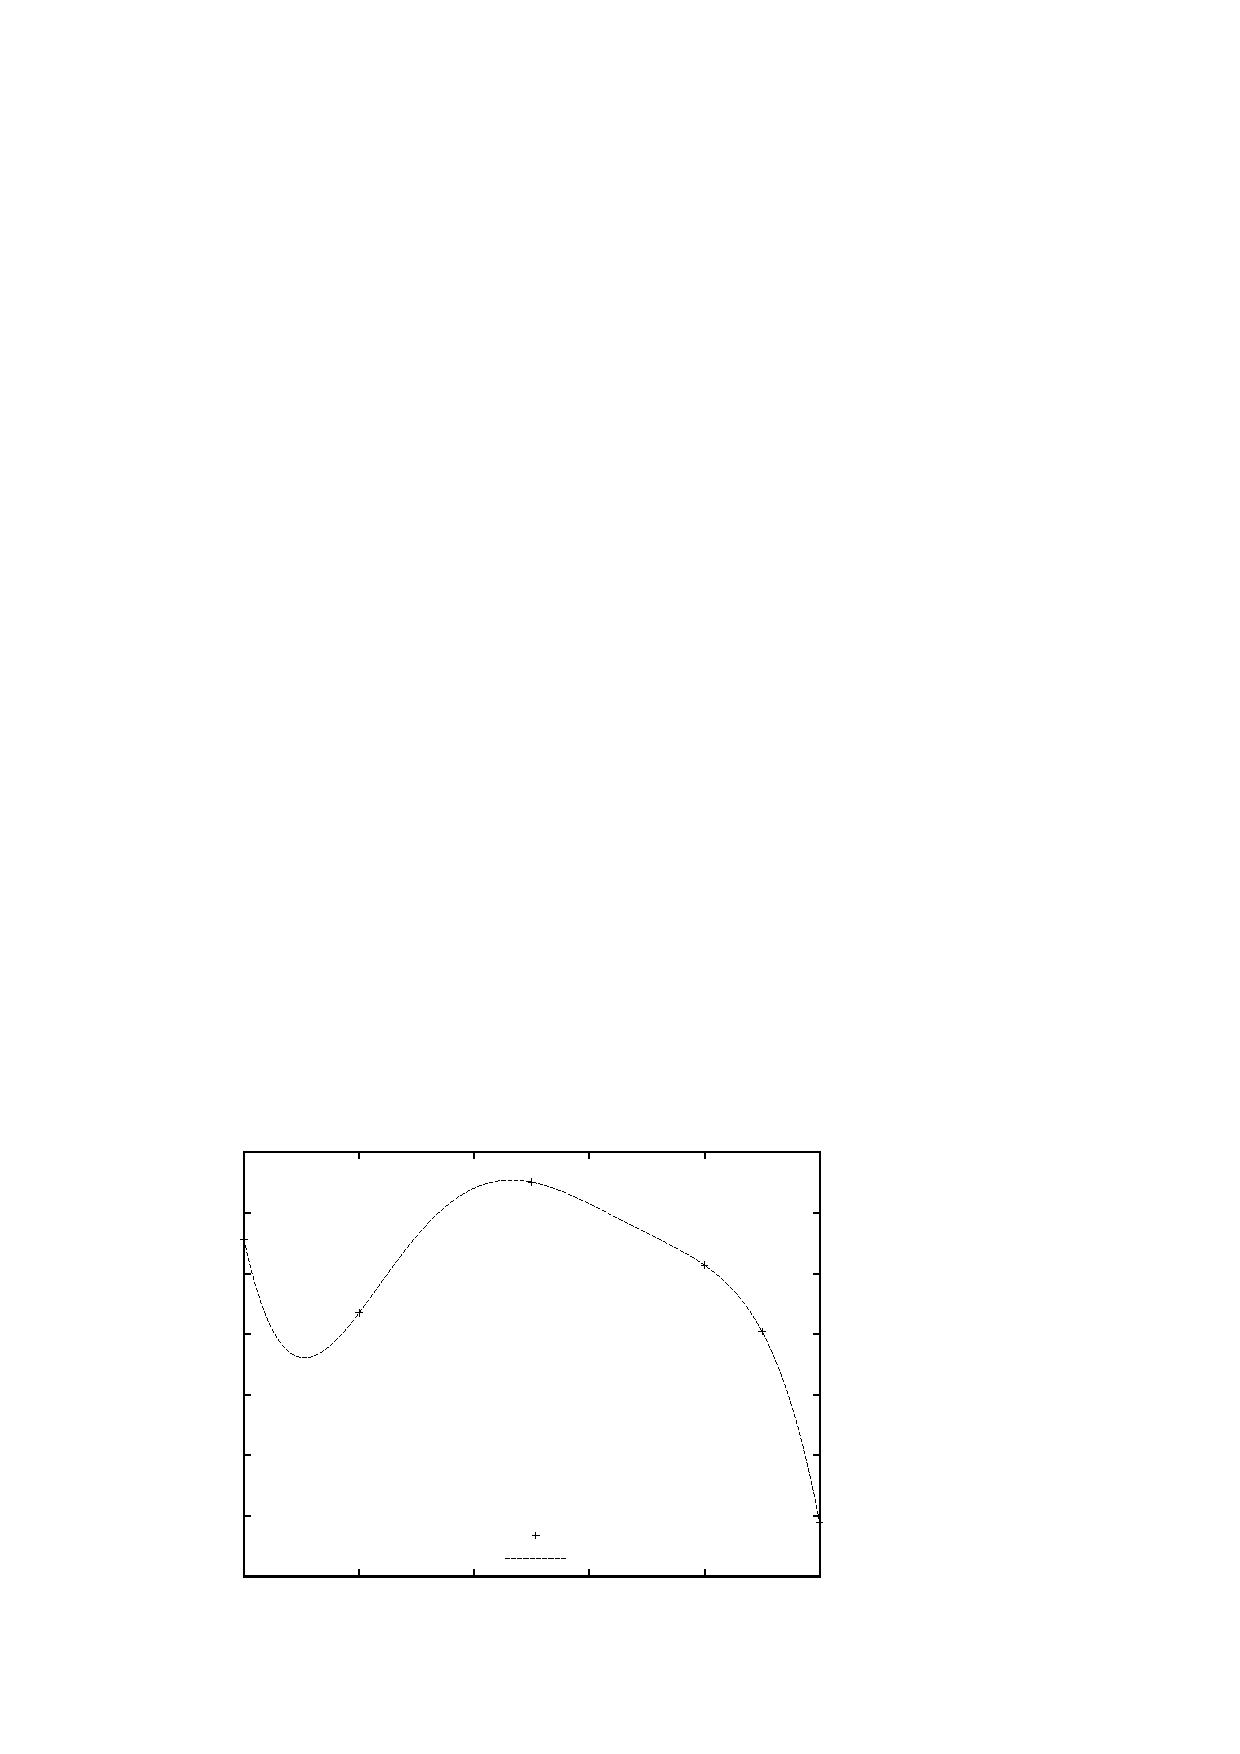
\includegraphics{G1}}%
    \gplfronttext
  \end{picture}%
\endgroup

\caption{Graf závislosti výtěžku rentgenového záření na atomovém čísle.}
\label{G1}
\end{figure}

\subsection{Slitiny}
Dále jsem proměřil vzorky 5 a 13, které byli slitinami. Výsledky měření jsou v tabulce \ref{TSlitiny}. Následně jsem určil relativní zastoupení kovů ve slitině 13 (Pb+Sn), k čemuž jsem využil hodnot naměřených u čistých kovů. Chyba intenzity je v případě první slitiny 1.4 procenta, v případě druhé 1.1 procenta. Výsledný poměr Sn:Pb je 2:3.

\begin{table}
$$
\begin{array}{|c|c|c|c|}
\hline
&   E/\mbox{keV}&   E_t/\mbox{keV}&   \frac{S}{t}/\mbox{cps} \\ \hline
5 Ag+Zn&&& \\ \hline
K_{Ag\alpha}& 22.18\pm 0.34&   22.159&   28.37 \\ \hline
K_{Ag\beta}& 25.03\pm 0.37&   24.938&   8.98 \\ \hline
K_{Zn\alpha + \beta}& 8.41\pm 0.46&   8.615&   4.54 \\ \hline
13 Pb+Sn&&& \\ \hline
K_{Sn\alpha}& 25.28\pm 0.42&   25.267&  28.7 \\ \hline
K_{Sn\beta}& 28.63\pm 0.35&   28.481&   4.81 \\ \hline
K_{Pb\alpha}& 10.62\pm 0.31&   10.550&   10.23 \\ \hline
K_{Pb\beta}& 12.70\pm 0.35&   12.612&   9.48 \\ \hline
\end{array}
$$
\caption{Výslednky měření spektra pro slitiny.}
\label{TSlitiny}
\end{table}

\subsection{Radioizotop}
Nakonec jsem proměřil spektrum radioaktivního zářiče. To odpovídalo Cs, které vzniká elektronovým záchytem z $^{133}$Ba. 
Naměřené hodnoty jsou v tabulce \ref{TRadio}.

\begin{table}
$$
\begin{array}{|c|c|c|c|}
\hline
&   E/\mbox{keV}&   E_t/\mbox{keV}&   \frac{S}{t}/\mbox{cps} \\ \hline
K_{Cs\alpha}&   30.90\pm 0.42&   30.968&   1256.35 \\ \hline
K_{Cs\beta}&    35.08\pm 0.43&  34.981&   314 \\ \hline
\end{array}
$$
\caption{Výslednky měření spektra pro radioizotop.}
\label{TRadio}
\end{table}
\section{Diskuze}
Naměřené hodnoty píků seděli na tabelových hodnotách dokonce o řád přesněji, než byla chyba určená z jejich pološířek. Díky tomu mlžeme s dobrou jistotoou říci, že při určení prvku vzorku nedošlo k chybě. Na jistotě přidává fakt, že rozdíly mezi hodnotami jednotlivých prvků jsou běžně o řád vyšší než chyba měření. 

Jedinou problematickou hodnotou měření mohla být $K_\beta$ u Zr, protože se velmi blízko kalibračního spektra Am. Tento pík se však díky uspořádání experimentu posunul až k hodnotám okolo 17.2 keV a tak nedošlo k žádnému překryvu těchto píků. 

Vzorek dvanác byl pouze kvalitativně určen, protože měření neposkytlo žádná validní data pro určení. Jednalo se o železo.

Pro určení poměru prvků ve slitině jsem zvolil vzorek 13, protože bylo možné využít již naměřených hodnot, což vedlo k nižší chybě, než jaká by vznikla při určování u vzorku 5.

Radioizotop se nechal určit velmi dobře, díky jeho výrazně vyšší intenzitě, než u kovů určovaných před tím.

\section{Závěr}
Zkalibroval jsem spektrometr za pomoci Am a jeho spektra. \\
Určil jsem vzorky kovů i slitin. Výsledky jsou v tabulkách \ref{TKovy} a \ref{TSlitiny}.
Sestrojil jsem graf závislosti výtěžku rentgenového záření na atomovém čísle, který je na obrázku (\ref{G1}). \\
Závislost jsem proložil polynomme pátého stupně, jehož předpis je uveden výše. \\
Určil jsem poměr zastoupení prvků ve vzorku 13, který je Sn:Pb=2:3. \\
Určil jsem ratioizotop $^{133}$Ba, který se rozpadá elektronovým záchytem.


\begin{thebibliography}{5}
	\bibitem{text} \textbf{Studijní text na praktikum IV} \\http://physics.mff.cuni.cz/vyuka/zfp/txt\_403.pdf (17. 12. 2012)
\end{thebibliography}


\end{document}
